% !TeX spellcheck = en-US
% !TeX encoding = utf8
% !TeX program = pdflatex
% !BIB program = biber
% -*- coding:utf-8 mod:LaTeX -*-


% vv  scroll down to line 200 for content  vv


\let\ifdeutsch\iffalse
\let\ifenglish\iftrue


\input{pre-documentclass}
\documentclass[
  %
  %ngerman, %%% Add if you write in German.
  %
  % fontsize=11pt is the standard
  a4paper,  % Standard format - only KOMAScript uses paper=a4 - https://tex.stackexchange.com/a/61044/9075
  twoside,  % we are optimizing for both screen and two-side printing. So the page numbers will jump, but the content is configured to stay in the middle (by using the geometry package)
  bibliography=totoc,
  %               idxtotoc,   %Index ins Inhaltsverzeichnis
  %               liststotoc, %List of X ins Inhaltsverzeichnis, mit liststotocnumbered werden die Abbildungsverzeichnisse nummeriert
  headsepline,
  cleardoublepage=empty,
  parskip=half,
  %               draft    % um zu sehen, wo noch nachgebessert werden muss - wichtig, da Bindungskorrektur mit drin
  draft=false
]{scrbook}
\input{config}


\usepackage[
  title={Visualizing Sleep Wellness: Data Physicalization as a Motivational Tool}, % Do not forget to capitalize your title correctly, you may use the following page to help you: https://capitalizemytitle.com/
  author={Marcus Reiners},
  email={marcus.reiners@campus.lmu.de},
  type=bachelor,
  institute={Institut für Informatik}, % or other institute names - or just a plain string using {Demo\\Demo...}
  course={Medieninformatik},
  examiner={Prof.\ Dr.\ Sven Mayer},
  supervisor={Henrike Weing\"artner,\ M.Sc.\\Luke Haliburton,\ M.A.Sc.},
  startdate={November 23, 2022},
  enddate={March 23, 2022},
  % Falls keine Lizenz gewünscht wird bitte auf "none" setzen
  % Die Lizenz erlaubt es zu nichtkommerziellen Zwecken die Arbeit zu
  % vervielfältigen und Kopien zu machen. Dabei muss aber immer der Autor
  % angegeben werden. Eine kommerzielle Verwertung ist für den Autor
  % weiter möglich.
  copyright=ccbysa, % ccbysa, ccbynosa, cc0, none
  language=english
]{lmu-thesis-cover}

\input{acronyms}

\makeindex

\begin{document}

%tex4ht-Konvertierung verschönern
\iftex4ht
  % tell tex4ht to create picures also for formulas starting with '$'
  % WARNING: a tex4ht run now takes forever!
  
  %\Configure{$}{\PicMath}{\EndPicMath}{}
  %$ % <- syntax highlighting fix for emacs
  \Css{body {text-align:justify;}}

  %conversion of .pdf to .png
  \Configure{graphics*}
  {pdf}
  {\Needs{"convert \csname Gin@base\endcsname.pdf
      \csname Gin@base\endcsname.png"}%
    \Picture[pict]{\csname Gin@base\endcsname.png}%
  }
\fi

%\VerbatimFootnotes %verbatim text in Fußnoten erlauben. Geht normalerweise nicht.

\input{commands}
\pagenumbering{arabic}
\Coverpage
\Copyright
%Eigener Seitenstil fuer die Kurzfassung und das Inhaltsverzeichnis
\deftriplepagestyle{preamble}{}{}{}{}{}{\pagemark}
%Doku zu deftriplepagestyle: scrguide.pdf
\pagestyle{preamble}
\renewcommand*{\chapterpagestyle}{preamble}



%Kurzfassung / abstract
%auch im Stil vom Inhaltsverzeichnis
\section*{Kurzfassung}

<Short summary of the thesis>

\cleardoublepage

\section*{Abstract}

<Short summary of the thesis>

\cleardoublepage


% BEGIN: Verzeichnisse

\iftex4ht
\else
  \microtypesetup{protrusion=false}
\fi

%%%
% Literaturverzeichnis ins TOC mit aufnehmen, aber nur wenn nichts anderes mehr hilft!
% \addcontentsline{toc}{chapter}{Literaturverzeichnis}
%
% oder zB
%\addcontentsline{toc}{section}{Abkürzungsverzeichnis}
%
%%%

%Produce table of contents
%
%In case you have trouble with headings reaching into the page numbers, enable the following three lines.
%Hint by http://golatex.de/inhaltsverzeichnis-schreibt-ueber-rand-t3106.html
%
%\makeatletter
%\renewcommand{\@pnumwidth}{2em}
%\makeatother
%
\tableofcontents

% Bei einem ungünstigen Seitenumbruch im Inhaltsverzeichnis, kann dieser mit
% \addtocontents{toc}{\protect\newpage}
% an der passenden Stelle im Fließtext erzwungen werden.

\listoffigures
\listoftables

% Control List of Listings
\let\iflistings\iffalse
%Wird nur bei Verwendung von der lstlisting-Umgebung mit dem "caption"-Parameter benoetigt
%\lstlistoflistings
%ansonsten:
\iflistings
  \ifdeutsch
    \listof{Listing}{Verzeichnis der Listings}
  \else
    \listof{Listing}{List of Listings}
  \fi
\fi

% Control List of Algorithms
\let\ifalgorithms\iffalse
\ifalgorithms
  %mittels \newfloat wurde die Algorithmus-Gleitumgebung definiert.
  %Mit folgendem Befehl werden alle floats dieses Typs ausgegeben
  \ifdeutsch
    \listof{Algorithmus}{Verzeichnis der Algorithmen}
  \else
    \listof{Algorithmus}{List of Algorithms}
  \fi
  %\listofalgorithms %Ist nur für Algorithmen, die mittels \begin{algorithm} umschlossen werden, nötig
\fi

% Control Glossary
\let\ifglossary\iffalse
\ifglossary
  \printnoidxglossaries
\fi

\iftex4ht
\else
  %Optischen Randausgleich und Grauwertkorrektur wieder aktivieren
  \microtypesetup{protrusion=true}
\fi

% END: Verzeichnisse


% Headline and footline
\renewcommand*{\chapterpagestyle}{scrplain}
\pagestyle{scrheadings}
\pagestyle{scrheadings}
\ihead[]{}
\chead[]{}
\ohead[]{\headmark}
\cfoot[]{}
\ofoot[\usekomafont{pagenumber}\thepage]{\usekomafont{pagenumber}\thepage}
\ifoot[]{}


%% vv  scroll down for content  vv %%














%%%%%%%%%%%%%%%%%%%%%%%%%%%%%%%%%%%%%%%%%%%%%%%%%%%%%%%%%%%%%%%%%%%%%%%%%%%%%%
%
% Main content starts here
%
%%%%%%%%%%%%%%%%%%%%%%%%%%%%%%%%%%%%%%%%%%%%%%%%%%%%%%%%%%%%%%%%%%%%%%%%%%%%%%


\chapter{Introduction}
\label{sec:introduction}

Sleep is not merely a habit but an essential requirement for the survival of an organism, similar to the necessity of adequate air, food, and fluid intake. It plays a vital role in promoting overall well-being by exerting a significant influence on both our physical and mental health. Extensive scientific research has consistently underscored the crucial importance of obtaining enough sleep, and it should not be underestimated \cite{Define_Sleep_Health}.

 Consequently, a deficiency in obtaining sufficient and restorative sleep can serve as a catalyst for numerous diseases. This includes mental repercussions like mood swings and cognitive impairment, as well as more severe physical consequences, such as the development of cardiovascular diseases, obesity, compromised immune function, and subsequently, an elevated risk of mortality \cite{Mortality_short_sleep, consequences_sleep_deprivation}. However, the fast-paced nature of modern society, together with the ubiquitous influence of technology and especially smartphones, have given rise to a range of sleep-related challenges that impact individuals’ sleep patterns and quality \cite{problematic_smartphone_use}. Consequently, improving sleep health has emerged as a critical public health necessity, bringing innovative approaches that bring individuals the opportunity to monitor, understand, and enhance their sleep behaviors effectively.

While various technological solutions, such as sleep tracking devices and applications, offer the promise of monitoring sleep, they often fall short in terms of motivating and engaging users to keep on tracking their sleep data. The abstract nature of the data presented by these tools can be challenging to interpret and act upon, impeding users' ability to make decisions based on their sleep data, to improve their sleep habits \cite{Sleep_essential_to_health}.
Furthermore, these data representations are most of the time hard to access through the use of personal devices like smartphones and tablets, pushing users to actively engage in specific actions to unveil their data \cite{Ambient_visualization}. In a study by  Li et al. \cite{Stage_Based_Model} it was observed that individuals who were using sleep tracking devices frequently often didn't take the time to review their gathered data. Consequently, this lack of engagement hinders users from obtaining a comprehensive perspective of their sleep data, thus impeding their ability to use it for self-reflection and behavior improvements \cite{Stage_Based_Model}. 

This study sets out to tackle the motivational gaps in sleep tracking through a physical representation of the gathered sleep data in an ambient way. This data physicalization involves the transformation of intangible sleep data into tangible and sensory representations, utilizing visual elements to enhance user engagement and comprehension \cite{Oppotunieites_Challenges_DataPhysicalization}. Previous research has indicated the potential effectiveness of using ambient information as a tool to minimize the level of attention required for the system interaction and to encourage user engagement \cite{Fostering_Engagement, Econundrum, Roam-IO}.
Therefore, the approach of an ambient visualization of data can help the integration of sleep data into the daily routine, making it an effortless component of everyday life.

While this technique has been previously employed in various domains, such as visualizing activity data \cite{LOOP, Shelfie, 10_Design_Themes, TastyBeats, Activity_Scupltures}, its application to the field of sleep health remains largely unknown. This research aims to explore the potential of data physicalization within the realm of sleep wellness, with a focus on bridging the gap between raw sleep data and user engagement. By delving into physical data representations, the study seeks to motivate individuals to take proactive steps towards better sleep health.

This research is organized in three main phases: initially, gathering user insights through an online survey to discern preferences and expectations, leading into a focus group to gather detailed expectations towards the object by individuals; subsequently, developing a prototype that harnesses ambient information to motivate and guide users on their path to improved sleep wellness.

Since a tendency towards a calming, relaxing and atmospheric design for a prototype emerged from the survey, we decided to use a candle as a form of data physicalization. Candles have been used frequently in studies in the past as a form of relaxation \cite{Candle_as_relaxation, Candle_reduce_stress} and are generally considered a calming and atmospheric illuminant. The features of this candle are used to display a total of three different sleep tracking records. An LED lamp is used to recreate the flame of the candle, which displays the overall sleep quality by flickering, and the sleep duration by brightness. The body of the candle consists of four displays, which show the sleep phases of the last night by colored bars. In order to also be able to collect this sleep data, in addition to an ordinary smartwatch, an app is used which consistently reads the collected data from the watch and stores it in a cloud, where the data is then loaded and read from there by the prototype.

The results of this study show initial attempts for the potential of data physicalization to make the representation of sleep data more approachable and less cumbersome. Thus, not only can the field of data visualization be expanded, but also the way people perceive, interact with, and prioritize their sleep health accordingly. By combining data, design, and user experience, this study is expected to pave the way for future studies with creative solutions that allow individuals to make informed decisions regarding their sleep behaviors. These findings could represent a new step towards understanding sleep behavior and, along with further research in the future, could change the perspective of various aspects of health and wellness behavior in today's society.

%This is a typical human-computer interaction thesis structure for an introduction which is structured in four paragraphs as follows:
% First Paragraph
% CORE MESSAGE OF THIS PARAGRAPH:
%\todo{P1.1. What is the large scope of the problem?}
%-Sleep-related issues and their impact on overall well-being
%\newline
%-Lack of effective motivational tools for individuals to monitor and improve their sleep
%\todo{P1.2. What is the specific problem?}
%-The limited exploration of Sleep Data-Physicalization
% Second Paragraph
% CORE MESSAGE OF THIS PARAGRAPH:
%\todo{P2.1. The second paragraph should be about what have others been doing}
%-Data Physicalization of Activity-Data
%\todo{P2.2. Why is the problem important? Why was this work carried out?}
%-Sleep health is a significant concern in modern society
%\newline
%-Lack of tools to engage and motivate individuals in prioritizing their sleep
% Third Paragraph
% CORE MESSAGE OF THIS PARAGRAPH:
%\todo{P3.1. What have you done?}
%-conducted two online surveys to find a desired Design approach
%\newline
%-Develop and test a Prototype
%\todo{P3.2. What is new about your work?}
%-Exploration of data physicalization as a means to engage and motivate users in their sleep wellness
% Fourth paragraph
% CORE MESSAGE OF THIS PARAGRAPH:
%\todo{P4.1. What did you find out? What are the concrete results?}
%\todo{P4.2. What are the implications? What does this mean for the bigger picture?}

%LaTeX hints are provided in \autoref{chap:latexhints}.

\chapter{Related Work}

This chapter provides an overview of the literature on the importance of sleep, sleep tracking and visualization techniques, and how data physicalization can be used as a motivational tool.
Sleep is an important component of human well-being, and understanding and improving sleep quality is of great interest in both medical and personal contexts. This section reviews the existing literature on health data visualisation and the use of data physicalisation as a motivational tool.

\section{Importance of Sleep}

Sleep, as one of the fundamental pillars of a healthy life, has gained substantial attention in both medical and personal contexts. Traditionally centered on addressing sleep disorders and insufficient sleep duration, the concept of sleep health now encompasses the whole well-being of individuals or entire populations \cite{Define_Sleep_Health}. Its significance as a foundation of health underscores the need to comprehensively understand and improve sleep quality.

\paragraph{Brain Functioning}
Sleep is essential for various physiological functions, particularly impacting the brain by playing a role across a variety of these functions \cite{tai_impact_2022}. A collection of articles elucidates the dynamic nature of sleep, its evolution across the lifespan, and its role in memory consolidation and integration \cite{simon_functions_2022}. Sleep re-energizes the body’s cells, clears waste from the brain, and supports learning and memory, although more research is needed to fully understand its role in mood, appetite, and libido regulation \cite{cirelli_sleeping_2017}. Emerging evidence suggests that a crucial function of the sleeping brain is the removal of wastes and toxins from the central nervous system due to the activation of the brain waste removal system \cite{semyachkina-glushkovskaya_brain_2023}. During non-rapid eye movement (REM) sleep, neural activity coupled with changes in blood volume enables cerebrospinal fluid to flow in slow waves; this process may help clear toxins from the brain that have been linked to neurodegenerative diseases \cite{lehmann_slow_2019}.

\paragraph{Growth and Repair}
Sleep is vital for cellular, organic, and systemic functions of an organism, affecting various physiological processes including hormonal axes \cite{dattilo_sleep_2011}. The function of sleep for repair or clearance becomes more pronounced during late ontogeny (after 2 or 3 years in humans) as shown by a quantitative analysis \cite{cao_unraveling_2020}. Sleep plays a role in neural reorganization and growth, significantly impacting the brain's structure and function, especially in infants and children \cite{brinkman_physiology_2023}.

\subsection{Consequences of Sleep Deprivation.}
Insufficient sleep duration and low sleep quality come together with a number of adverse health effects. The adverse effects of insufficient sleep duration, sleep apnoea and insomnia on various aspects of health such as mortality, weight loss, diabetes, inflammation, cardiovascular health, cognitive function and psychological well-being have been extensively described in the literature \cite{Sleep_Health_Society}.

\paragraph{Mortality}
Sleep deprivation has been associated with increased all-cause mortality, particularly in men. Several mechanisms have been suggested to explain this association. For instance, sleep restriction during the night can alter endocrine and metabolic function, which may in turn be implicated with mortality or cardiovascular events \cite{yin_relationship_2017}. Laboratory data support a link between short sleep duration and physiological and social outcomes which could relate to mortality \cite{grandner_mortality_2010}.

\paragraph{Weight Loss}
Sleep deprivation can significantly affect weight loss efforts and maintenance. It has been found to alter eating habits, metabolic rate, and the hormones regulating metabolism, which are all crucial factors for weight management \cite{papatriantafyllou_sleep_2022}. Moreover, sleep deprivation is associated with weight gain and obesity as it can increase appetite, reduce feelings of fullness after eating, and make individuals more likely to reach for junk foods \cite{chamorro_sleep_2011}.

\paragraph{Cardiovascular Health}
Sleep deprivation is associated with an elevated risk of cardiovascular issues, such as hypertension and coronary heart disease. Insufficient sleep, marked by less than 7 hours per night, tends to exacerbate existing cardiovascular conditions. The underlying mechanisms include endothelial dysfunction and disrupted signaling pathways leading to cardiac incidents \cite{belloir_sleep_2022}

\paragraph{Cognitive Functions (Accidents)}
The consequences of sleep deprivation have a detrimental impact on neurobehavioral functioning \cite{durmer2005neurocognitive,lim2008sleep,lim2010meta} and result in heightened daytime fatigue and drowsiness, increasing the likelihood of accidents stemming from human errors \cite{axelsson2008sleepiness, dinges1995overview}. Sleep deprivation leads to cognitive and motor performance impairments comparable to those induced by alcohol consumption at or above the legal limit \cite{williamson2011link}. Drowsy driving incidents are widespread, with 32\% of participants in the 2008 National Sleep Foundation Sleep in American Poll admitting to having driven while drowsy, and 36\% acknowledging brief episodes of nodding off while driving in the past year. Drowsy driving significantly contributes to a notable portion of traffic accidents, accounting for up to 20\% of cases \cite{williamson2000moderate}. Beyond the elevated risk of motor vehicle collisions, sleep deprivation and the resultant drowsiness are associated with occupational injuries and fatal accidents \cite{connor2001role, aakerstedt2002prospective}. These severe consequences underscore the irreplaceable necessity of sleep and its pivotal role in society at large.

\section{Sleep Tracking and Visualizations}
The public availability of sleep tracking technologies has introduced new opportunities for individuals to monitor their sleep well-being \cite{Challenges_Oppotunieties_SleepTracking}. Originally conceived for scientific research, these technologies now give users the opportunity to gain insights into their sleep patterns and habits.
\paragraph{Sleep Tracking Technologies}
Sleep tracking technologies have gained considerable interest in recent years as valuable tools for monitoring and assessing sleep patterns. These technologies utilize various sensors and devices to collect data on an individual's sleep duration, sleep stages, movement, and environmental factors. Consumer-oriented devices like a wearable fitness tracker or a smartphone app have the potential to enhance overall sleep well-being, by measuring the sleep duration, giving a rating of the overall sleep quality, and waking the user during light sleep phases \cite{Consumer_SleepTracking}. However, the question of whether these technologies can truly improve sleep remains subtle.

\paragraph{Impact of Sleep Tracking.}

The study "Smartphone applications for sleep tracking: rating and perceptions about behavioral change among users" found that 30-50\% of participants believed sleep tracking apps increased awareness about sleep patterns and hygiene, influenced sleep hygiene habits, and encouraged help-seeking when needed. However, it also noted the need for improved quality and content in these apps, as the average app quality score was 3.3 out of 5 \cite{karasneh_smartphone_2022}. Sleep tracking predominantly enhances awareness of sleep patterns. However, it's unclear if this awareness translates to sleep improvement due to barriers like a lack of reference points for data interpretation, inaccuracies in sleep data, and a lack of motivational elements within the tracking systems to encourage actionable steps towards better sleep hygiene \cite{SleepTracking_in_the_real_world}.

\paragraph{Sleep Visualization Techniques}
Visualizing sleep data is essential for understanding sleep patterns . Consumer sleep tracking devices lack standardization and often use proprietary algorithms, relying on built-in accelerometers to define sleep parameters \cite{SleepTracking_ClnicalCare, lee_consumer_review2015}. These devices offer the advantage of measuring sleep quality in natural environments \cite{Making_sense_of_sensors}. User adherence to tracking, or how regularly data is collected, can affect perceived accuracy \cite{Defining_Adherence}. However, user perception of accuracy is not always based on technical validation.
Users have concerns about data trustworthiness, including variations between devices and doubts about sleep recognition \cite{Challenges_Oppotunieties_SleepTracking}. Subjective perceptions of sleep quality, such as how much sleep is enough to feel rested, can lead to a discomfort between metrics and user experience \cite{sleepexplorer}. Lack of trust in captured data reduces user acceptance \cite{Trust_activity_tracker} and may challenge long-term device adoption \cite{sleepexplorer}. Unrealistic expectations about device capabilities can also affect the perception accuracy \cite{Use_and_Adoption}.
Some users may not change their sleep habits despite tracking data due to a lack of understanding of normal sleep and uncertainty about improvement \cite{SleepTracking_in_the_real_world}. Liang et al. suggest design considerations related to data accuracy, visualization, guidance, and personalized recommendations to address these issues \cite{SleepTracking_in_the_real_world}.

\section{Data Physicalization as a Motivational Tool}
A data physicalization is a physical artifact whose geometry or material properties encode data. Physicalization is an innovative approach to visualizing data using tangible, three-dimensional models. The original definition, proposed by Jansen et al., emphasized that only the physical characteristics of the artifact hold the encoded data \cite{Oppotunieites_Challenges_DataPhysicalization}. However, Hogan and Hornecker expanded this definiton by asserting that data can also be encoded not only in the shape but also in the behavior of the physical representation \cite{Representation_Modality_Data_Artifacts}.
Dynamic physicalization involves interactive and responsive visualizations using tangible models. Users can manipulate the physical objects to explore specific data points or regions of interest while observing real-time changes \cite{Oppotunieites_Challenges_DataPhysicalization}. This broader perspective of data physicalization highlights the significance of considering the object's materiality and its quality of presence in the world, a concept well-studied in design research \cite{Structures_Forms_Stuff_Interaction, Materiality_of_interaction}. It acknowledges that data physicalization goes beyond mere representation and encompasses a holistic view. Furthermore, Offenhuber's perspective challenges the conventional notion of data by emphasizing that data physicalization can extend beyond external datasets \cite{Talk_About_Physicality}.
\paragraph{Ambient Information}
Ambient information systems, requiring minimal attention and cognitive effort, have been designed to motivate individuals towards healthier behaviors like regular exercise. These systems employ strategies like abstraction, historical information reflection, and triggers to motivate users towards desired actions \cite{rodriguez_cammina_2013}. For instance, in a work environment, an ambient information system was developed using a sensor-actuator system, to provide a responsive office setting, which was evaluated by experimental participants for its impact \cite{streitz_ambient_2023}. Similarly, ambient mirrors have been used to reflect a user's current behavior or attitude, supporting behavior change through personalized feedback, with one case study showcasing the reflection of a user's physical exercise status in artistic images \cite{nakajima_designing_2013}.
These examples underline the potential of integrating ambient information systems in sleep wellness programs to motivate individuals towards better sleep hygiene and overall sleep quality improvement.

\section{Summary}
This section has provided an overview of the existing literature related to sleep health, sleep tracking technologies, visualization techniques, and the emerging field of data physicalization. The subsequent sections will build upon those insights to explore the integration of data physicalization as a motivational tool within the context of sleep wellness.


\chapter{Methodology}

This chapter provides an overview of the research methods used in this thesis. The research process consists of three phases, each of which contributes to the overall investigation. Previous research on the use of data physicalisation as a motivational tool shows a clear gap regarding the application and implementation of ambient designs to make captured sleep data more accessible to users.
There are already approaches in data recording through fitness trackers, such as the display of daily step count \cite{LOOP}. However, despite the serious implications of insufficient sleep quality and duration \cite{Sleep_Health_Society}, the implementation of data physicalization in the context of sleep data remains largely unexplored. With this in mind, we wanted to make sleep more tangible, increase users' awareness of their sleep patterns and well-being, and motivate them to adopt healthier habits.

Before proceeding with the selection of a research methodology, we formulated three research questions to ensure alignment with the objectives of our project:

\begin{itemize}
    \item \textbf{RQ1:} What categories of sleep data are relevant for effective visualisation and understanding to promote sleep wellness?
    \item \textbf{RQ2:} What design principles and elements should be incorporated into a prototype to effectively communicate sleep data to users?
    \item \textbf{RQ3:} What data communication methods should the prototype use to ensure accurate and understandable transmission of sleep data to users?
\end{itemize}

Since everyone needs enough sleep to survive, we wanted to collect results from an unrestricted target group. Therefore, in order to make our findings more widely applicable, we decided to conduct a quantitative survey, formulating questions based on the relevant research. The aim was to gain a deeper understanding of the relevant requirements in relation to the articulated research questions that would guide the prototyping process. After analyzing the survey results, we were able to make first design decisions for our tangible artifact. However, as the survey could not provide precise ideas, but only a rough theme, a focus group was then held to collect explicit design ideas from a diverse group and to inspire the design decisions of the prototype. These provided a framework for determining the mechanisms and aesthetics of the tangible object. We then started working on the prototype, including both software and hardware, and held weekly meetings to evaluate design choices and iteratively refine the system. The final step in achieving our project goal was to build the hardware of the prototype and make it tangible.

\subsection{Survey Phase:} 
The research began with a preliminary study on sleep tracking and sleeping habits. It also already served to gather initial ideas for a potential prototype design. In this first step, data from over 150 participants, without any restrictions, were collected and analyzed.

\subsection{Focus Group Phase}
Following the survey phase, a focus group was conducted, in order to build upon the gathered data from the online survey and also to have a few hands-on examples for a potential prototype. The focus group yielded valuable results for the research process, consolidating some of the findings from the online survey.

%this section is an overview of %the entire thesis
%- first doing survey
%- then focus group
%- then implementation
%- then evaluation

%this section only needs to be %like 0.5-1 page

\chapter{Online Survey}
\section{Method}
\subsubsection{Participants}
A total of 156 participants, mostly recruited via an e-mail distributor, attended for this study. The participants' demographics revealed a range of ages, with an average age of 28.53 years. The gender distribution was as follows: 86 female, 55 male, 4 preferred not to say, 3 identified as non-binary, and 2 with other gender identities.
\subsubsection{Survey Content}
During the online survey, participants were initially asked in detail about their sleep habits or any existing sleep disorders. Based on this, the previous use of sleep tracker devices was explored in more detail by asking, among other things, the actual frequency of use and the improvements in sleep habits that occurred or did not occur as a result. The main part of the study was to gather participants' ideas and perceptions for a potential prototype that would present collected sleep data as a data physicalization.


\section{Results}
\subsection{Sleep-Related Questions}

    \textbf{Sleep Disorders:} 36 participants reported having sleep disorders or conditions that affect their sleep, while 108 did not.
    
    \textbf{Factors Affecting Sleep:} 99 participants reported specific factors that impact the quality of their sleep, such as noise, temperature, and stress, while 45 did not.
    \textbf{Average Sleep Duration:} Participants reported an average sleep duration ranging from 3 to 12 hours, with a mean of 7.03 hours.
    \textbf{SATED Questionnaire}
    Participants responded to the Sleep Assessment in Daily Life (SATED) questionnaire, which evaluated various aspects of their sleep satisfaction, daytime alertness, and sleep duration.
    \begin{figure}
        \centering
        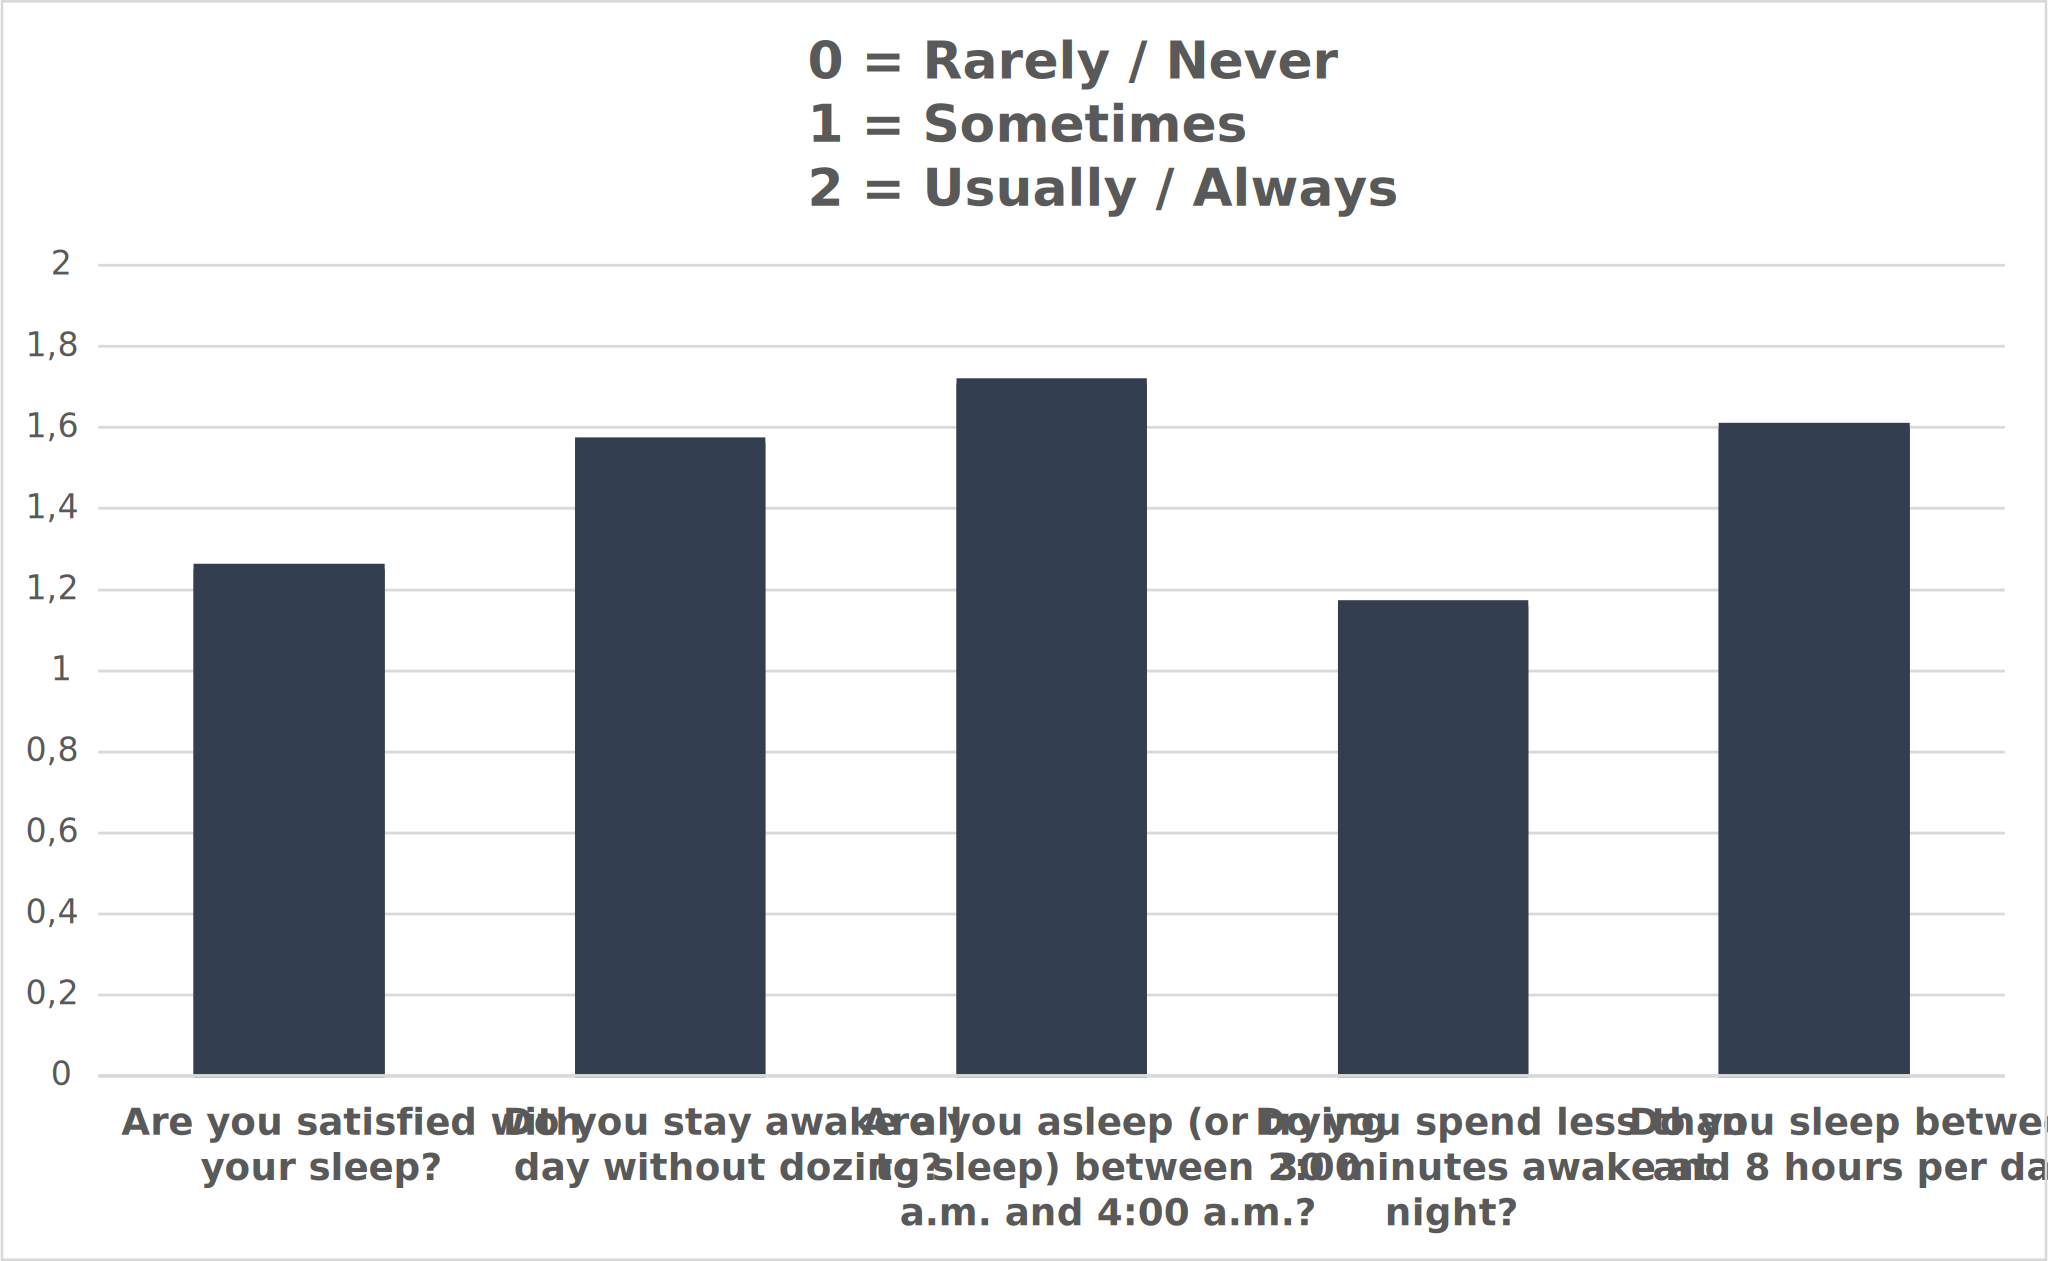
\includegraphics[scale = 0.2]{graphics/SATED_Charts.svg}
        \caption{SATED Questionnaire}
    \end{figure}

    \begin{figure}
        \centering
        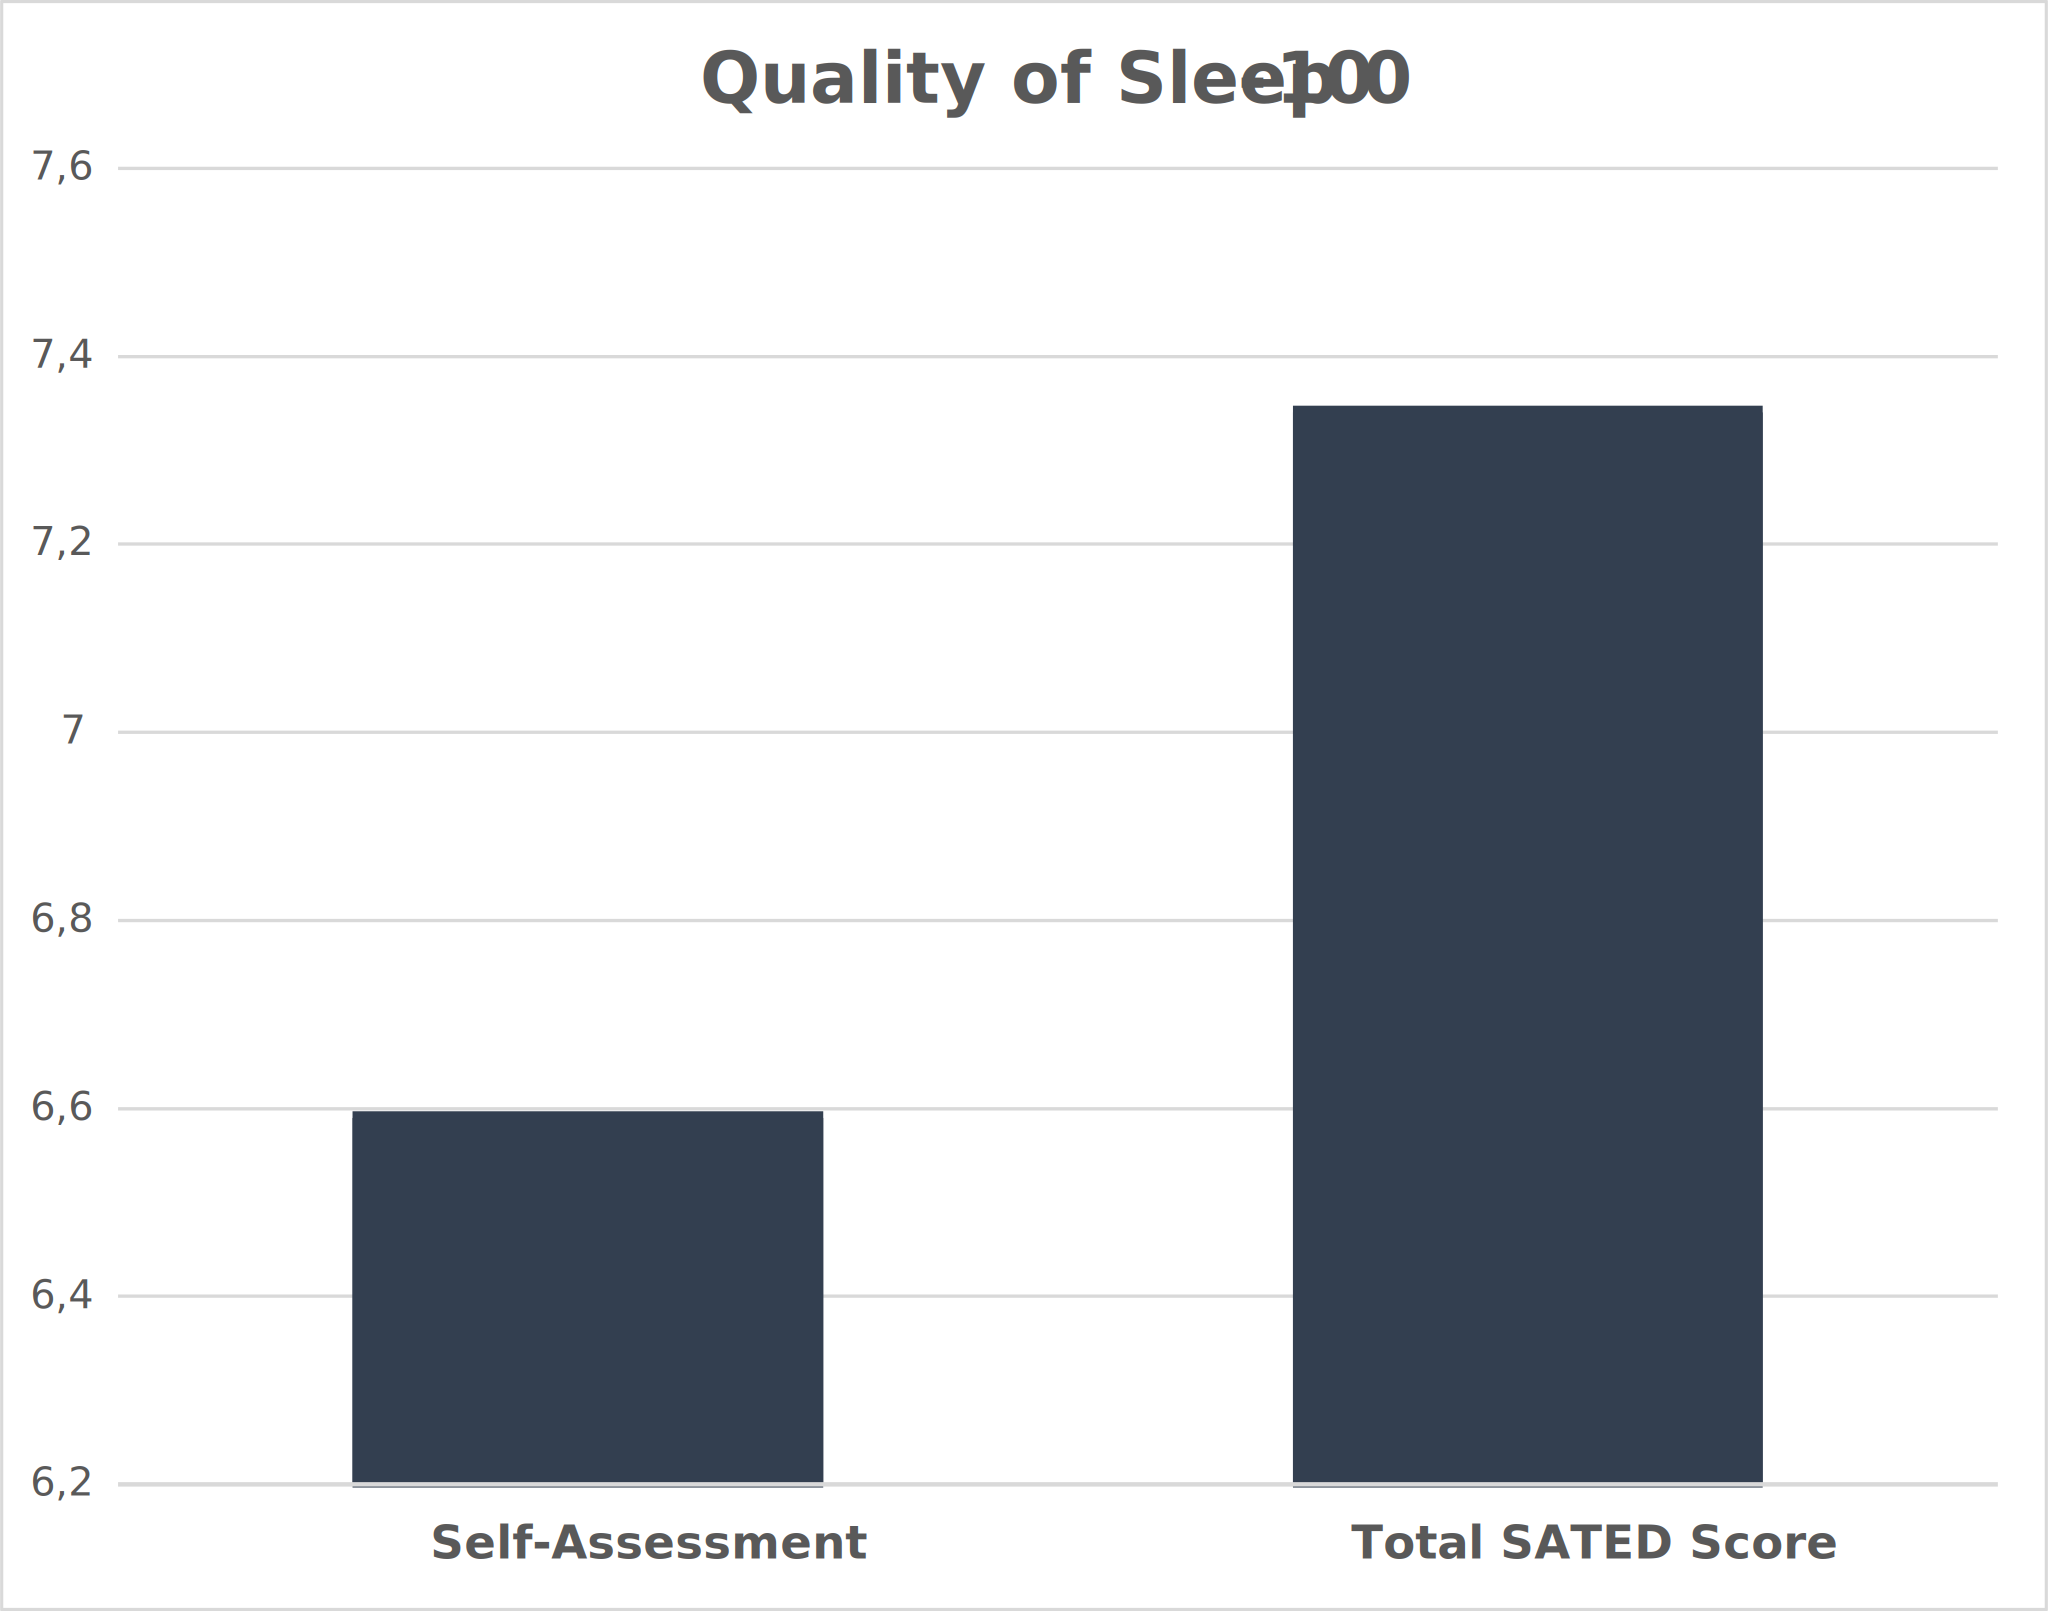
\includegraphics[scale=0.24]{graphics/SATEDvsSELF.svg}
        \caption{Self-Assessment and Total SATED Score}
    \end{figure}

    

    \textbf{Sleep Quality:} Participants rated their sleep quality on a scale from 0 to 10, with a mean score of 6.6.
    \textbf{Comparison with SATED Mean:} A comparison between participants' own perception and the results from the SATED questionnaire indicates that the participants are experiencing a better sleep quality compared to their own perception. Own perception sleep quality mean (6.6), SATED sleep quality mean (7.34).
    \textbf{Sleep Tracking:} A majority (89) reported never using health trackers to record their sleep, while 30 had used them in the past but discontinued use. Of those who discontinued use, reasons included lack of interest or perceived values, discomfort or inconvenience, forgetfulness, and other factors. 25 participants reported continued use of sleep trackers.


\subsection{Object Design Preferences}
    Participants were presented with questions related to the design of a physical object representing sleep data:

    \begin{itemize}
        \item \textbf{Things/Concepts Associated with Sleep:} Participants associated sleep with concepts such as rest, relaxation, and recovery.
        \item \textbf{Preferred Sleep Data for Visualization} The majority of participants indicated interest in visualizing sleep quality, sleep duration, and sleep stages.
        \item \textbf{Expected Insights:} Participants expected the object to help them understand sleep quality and efficiency, identify sleep disturbances, increase self-awareness of sleep habits, and motivate them to improve sleep.
        \item \textbf{Time Interval for Representation:} Daily and weekly representations were favored.
        \item \textbf{Interaction and Communication:} Participants preferred touch-based and light-based interaction and communication with the physical object.
        \item \textbf{Portability and Position:} Most participants preferred a portable object placed next to their bed, similar in size to a smartphone.
    \end{itemize}

\section{Online Survey Discussion}

\subsection{Important Concepts/Themes}
\begin{itemize}
    \item \textbf{Interest in sleep tracking:} The fact that participants showed interest in sleep tracking despite different sleep habits underlines the importance of developing a user-friendly and appealing device.
    \item \textbf{Sleep quality and satisfaction:} The participants' statements about their sleep quality and satisfaction, both from their own perceptions and via the SATED questionnaire, provide information about an incorrect self-assessment regarding their own sleep quality. This suggests that a device as an additional aid could provide a more accurate idea of actual sleep quality.
\end{itemize}

\subsection{Potential Objects:} 
\begin{itemize}
    \item 
\end{itemize}

\subsection{Placement (Where Should It Be):} 
The preference for a sleep tracking device that doesn't require participants to wear anything or be intrusive suggests that the prototype should be unobtrusive in the sleep environment. Consider placing it near the bed or in a location where it seamlessly integrates into the bedroom.
\subsection{Relevant Data:}
\begin{itemize}
    \item \textbf{Factors Affecting Sleep:} The specific factors mentioned by participants that affect their sleep (e.g., noise, temperature) could inform the type of data the prototype collects and presents. For example, if noise negatively impacts sleep, the prototype could include a noise monitoring feature.
    \item \textbf{Sleep Quality and Satisfaction:} Given the participants' focus on sleep quality and satisfaction, the prototype should provide meaningful data related to these aspects. This could include sleep scores, sleep duration, and other metrics that help users understand and improve their sleep quality.
    \item \textbf{Sleep Disorders:} For participants with sleep disorders, the prototype could offer specific features or recommendations tailored to their conditions, aiming to improve their sleep quality.
\end{itemize}

%What info from the survey can we use in designing the prototype
%- which concepts/themes are important
%- which potential objects
%- where should it be
%- how should it display info
%- which data?

\chapter{Focus Group}
\section{Method}
\subsubsection{Participants}

\begin{itemize}
    \item \textbf{Participant 1:} A researcher in the field of software engineering and machine learning
    \item \textbf{Participant 2:} Someone who has recently completed research at a different academic chair
    \item \textbf{Participant 3:} A research assistant from a different chair
    \item \textbf{Participant 4:} Another researcher who is actively involved in ongoing projects on the chair Human-Centered Ubiquitous Media
    \item \textbf{Participant 5:} A student who has experience with sleep disorders
    \item \textbf{Participant 6:} A Ph.D. student who is also active at the chair of Human-Centered Ubiquitous Media
\end{itemize}
\subsubsection{Survey Content}
This focus group aimed to further elaborate on the results of the online survey. Participants were actively encouraged to work together with tools to create or design a prototype that corresponds to their ideas for implementing a physical visualisation of sleep data. The participants were divided into three groups and after a short introduction they had about 30 minutes to develop a prototype. To help them, the participants were given some sleep tracking variables to use, such as sleep duration, sleep quality and sleep stages, which were also the most requested variables from the online survey. Of course, the participants were also allowed to use their own variables. As additional support, a guiding form was used, which, with the help of some specific questions regarding the prototype, could help to develop a well thought-out design.
\section{Results}
The focus group discussion generated some interesting concepts and themes that provided important guidance for the development of the sleep monitoring prototype. In general, there was a collective interest among participants in sleep monitoring methods, even though they do not currently monitor their own sleep. Some of the key points and findings from the focus group include:

\begin{itemize}
    \item \textbf{Interest in sleep tracking:} Participants were interested in the topic of sleep tracking, even if they do not do it themselves.
    \item \textbf{Comfort and portability:} An important theme that emerged was the desire for more comfort while sleep is being recorded. Participants preferred non-invasive solutions.
\end{itemize}
\section{Focus Group Discussion}
\subsection{Potential Objects}
Focus group participants had several ideas for potential objects to work as prototypes for sleep monitoring. These ideas are alternative suggestions of the design and could be explored further in future studies. They are the following ideas:

\begin{itemize}
    \item \textbf{Docking station:} In group 1, the participants proposed a two-part object, one is a docking station that can be placed next to the bed. The other additional object is a small portable ball connected to a string and a collection container. This object changes colour to indicate sleep stages and can be pressed to relieve stress. The length of the string changes according to the length of sleep, allowing successful play with the object only when there is enough sleep. It also warms up to signal bedtime and can act as an alarm light. The docking station, in turn, is responsible for charging the wearable sphere and also allows a more detailed view of the collected sleep data.
    \item \textbf{Integrated alarm clock:} In group 2, participants suggested integrating sleep monitoring into a common alarm clock. This device would project sleep data on the wall and include important statistics such as, colour-coded sleep quality, sleep duration and heart rate information. 
    \item \textbf{Interactive alarm clock:} In group 3, participants suggested an interactive wall clock. The hand of the clock indicates when certain sleep events occur and the entire mattress-shaped clock deforms according to the shape of the mattress at that time.
\end{itemize}

\subsection{Placement (Where Should It Be)}
Participants gave their preferences for the placement and portability of the prototype:

\begin{itemize}
    \item \textbf{Near the bed:} Similar to the online survey, in Group 1 and Group 2 participants suggested placing the prototype near the bed, for example on a bedside table.
    \item \textbf{Portability:} Several participants stressed the importance of portability. They wanted the device to be able to be placed in different places if they were not sleeping at home.
\end{itemize}

\subsection{Relevant Data}
Participants had different views on the relevance of the data:
\begin{itemize}
    \item \textbf{Data use:} Participants questioned how the data collected could be used. Some were concerned about whether the data could actually help improve sleep habits, especially if they already had good sleep routines.
    \item \textbf{Differentiation from smartphones:} Participants emphasized that the sleep monitoring prototype should offer something equivalent to functions that cannot be performed by a smartphone. This could be physical interactions or assistance in waking up.
\end{itemize}


%What info from the focus can we use in designing the prototype
%- which concepts/themes are important
%- which potential objects
%- where should it be
%- how should it display info
%- which data?

\chapter{Prototype Design}

\section{Design}
The design of the prototype aimed to create a sensory and intuitive representation of sleep data. Considering the participants' preferences for light-based interaction and non-intrusiveness, aligning with the study's goal of making sleep data accessible, engaging and comprehensible. After analyzing the results from the survey, we came up with the design of a candle, representing the participants' association of restfulness, relaxation and calmness towards sleep. Since most participants were interested in a visualization of especially the sleep quality, the sleep duration and the sleep stages, the candle is able to display those variables in a manner that embodies data physicalization principles. Sleep stages are communicated through a square alignment of four screens, with each screen displaying the same image. The images consist of colored bars stacked above each other, indicating the duration of each sleep stage. The candle is able to display following sleep stages: light sleep, deep sleep, REM, and awake. The sleep duration is communicated via a single LED on top of the candle representing the candles' flame. The brightness of the flame shows how healthiness of the slept duration by comparing the users sleep duration to a considered healthy amount of sleep hours. The flame also is able to communicate the users sleep quality by having a flickering flame. The more the flame is flickering the worse the tracked sleep quality. The overall sleep quality is calculated by comparing the presence of certain sleep stages and the actual sleep duration by considered healthy sleep habits. This choice reflects a holistic approach to visualizing sleep data that resonated with participants' expectations and preferences.

\section{Implementation}

\begin{figure}
    \centering
    \includegraphics[height=\paperheight, width=\paperwidth, angle=90, keepaspectratio]{graphics/InputOutput.drawio (3).pdf}
    \caption{Implementation and Interaction Layout Diagram}
    \label{fig:enter-label}
\end{figure}

\chapter{Discussion and Future Work}
\section{Discussion}
\section{Limitations}
\section{Future Work}

\chapter{Conclusion}


\printbibliography

All links were last followed on \today.

\appendix
%\input{latexhints/latexhints-english}

\pagestyle{empty}
\renewcommand*{\chapterpagestyle}{empty}
\Affirmation
\end{document}
